% Full instructions available at:
% https://github.com/elauksap/focus-beamertheme

\documentclass[9pt]{beamer}
\usetheme{focus}

%%%%%%%%%%%%%%%%%%%%%%%%%%%%%%%%%%%%%%%%%%%%%%%%%%%%%%%%%%%%%%%%%%%%%
% Typography, change document font
\usepackage[tt=false, type1=true]{libertine}
\usepackage[varqu]{zi4}
\usepackage[libertine]{newtxmath}
\usepackage[T1]{fontenc}

\usepackage[protrusion=true,expansion=true]{microtype}

% Disable paragraph indentation, and increase gap
\usepackage{parskip}

%Matrix
\usepackage{tabstackengine}
\setstackEOL{;}% row separator
\setstackTAB{,}% column separator
\setstacktabbedgap{1ex}% inter-column gap 
\setstackgap{L}{1.0\normalbaselineskip}% inter-row baselineskip
\let\mat\bracketMatrixstack

\newcommand{\pth}{Figure/}
\newcommand{\ve}[1]{\mathbf{#1}}

% Copyright (C) 2018-2019 Pasquale Claudio Africa and the LaTeX community.
% A full list of contributors can be found at
%
%     https://github.com/elauksap/focus-beamertheme
% 
% This file is part of beamerthemefocus.
% 
% beamerthemefocus is free software: you can redistribute it and/or modify
% it under the terms of the GNU General Public License as published by
% the Free Software Foundation, either version 3 of the License, or
% (at your option) any later version.
% 
% beamerthemefocus is distributed in the hope that it will be useful,
% but WITHOUT ANY WARRANTY; without even the implied warranty of
% MERCHANTABILITY or FITNESS FOR A PARTICULAR PURPOSE. See the
% GNU General Public License for more details.
% 
% You should have received a copy of the GNU General Public License
% along with beamerthemefocus. If not, see <http://www.gnu.org/licenses/>.

\mode<presentation>


% DEFINE COLORS. ---------------------------------------------------------------
\definecolor{main}{RGB}{134, 161, 174}
\definecolor{main2}{RGB}{104, 131, 144}
\definecolor{textc}{RGB}{20, 20, 20}
\definecolor{background}{RGB}{255, 255, 255}

\definecolor{alert}{RGB}{180, 0, 0}
\definecolor{example}{RGB}{0, 110, 0}


% SET COLORS. ------------------------------------------------------------------
\setbeamercolor{normal text}{fg=textc, bg=background}
\setbeamercolor{alerted text}{fg=textc}
\setbeamercolor{example text}{fg=textc}

\setbeamercolor{titlelike}{fg=background, bg=main}
\setbeamercolor{frametitle}{parent={titlelike}}

\setbeamercolor{footline}{fg=background, bg=main2}

\setbeamercolor{block title}{bg=main!80!background, fg=background}
\setbeamercolor{block body}{bg=main!10!background, fg=textc}

\setbeamercolor{block title alerted}{bg=alert, fg=background}
\setbeamercolor{block body alerted}{bg=alert!10!background, fg=textc}

\setbeamercolor{block title example}{bg=example, fg=background}
\setbeamercolor{block body example}{bg=example!10!background, fg=textc}

\setbeamercolor{itemize item}{fg=textc}
\setbeamercolor{itemize subitem}{fg=textc}

\setbeamercolor{enumerate item}{fg=textc!70!black}
\setbeamercolor{enumerate subitem}{fg=textc!70!black}

\setbeamercolor{description item}{fg=textc!70!black}
\setbeamercolor{description subitem}{fg=textc!70!black}

\setbeamercolor{caption name}{fg=textc}

\setbeamercolor{section in toc}{fg=textc}
\setbeamercolor{subsection in toc}{fg=textc}
\setbeamercolor{section number projected}{bg=textc}
\setbeamercolor{subsection number projected}{bg=textc}

\setbeamercolor{bibliography item}{fg=main}
\setbeamercolor{bibliography entry author}{fg=main!70!black}
\setbeamercolor{bibliography entry title}{fg=main}
\setbeamercolor{bibliography entry location}{fg=main}
\setbeamercolor{bibliography entry note}{fg=main}

\mode<all>


\begin{document}
	\tableofcontents
	
	\section{Two dimensional problems having a single variable : \today}
	\begin{frame}{Model equation}
		\begin{itemize}
			\item Suppose we are trying to find the solution $u(x,y)$ of the following partial differential equation
			\begin{equation}
			 -\frac{d}{dx}\left(a_{xx} \frac{\partial du}{\partial dx} + a_{xy} \frac{\partial u}{\partial y} \right)
			 -\frac{d}{dy}\left(a_{yx} \frac{\partial du}{\partial dx} + a_{yy} \frac{\partial u}{\partial y} \right) + a_{00} u = f(x,y) \quad \text{in} \quad \Omega
			\end{equation}	
			The coefficients are also a function o u : eg $a_{xx} = f(x,y,u,\frac{\partial u}{\partial x }, \frac{\partial u}{\partial y})$
			\item When we descritize it with $\bar{\Omega}$ with a boundary $\bar{\Gamma}$, we get a residual given as :
			\begin{equation}
				R(u_h) = 
				-\frac{d}{dx}\left(a_{xx} \frac{\partial du_h}{\partial dx} + a_{xy} \frac{\partial u_h}{\partial y} \right)
				-\frac{d}{dy}\left(a_{yx} \frac{\partial du_h}{\partial dx} + a_{yy} \frac{\partial u_h}{\partial y} \right) + a_{00} u = f(x,y)
			\end{equation}
		\end{itemize}
	\end{frame}


	\begin{frame}{Weak form}
		The step is to multiply the residual with the ith weight function $w_i(x,y)$ which should be differentiable too. We then set $w_iR$ over the element domain $\Omega^e = 0$
		\begin{itemize}
			\item $0 = \int_{\Omega_e} w_i \left[ 
			-\frac{d}{dx}\left(a_{xx} \frac{\partial u_h}{\partial x} + a_{xy} \frac{\partial u_h}{\partial y} \right)
			-\frac{d}{dy}\left(a_{yx} \frac{\partial u_h}{\partial x} + a_{yy} \frac{\partial u_h}{\partial y} \right) + a_{00} u - f(x,y) \right] dxdy$
			\item Now we know : $\frac{d}{dx}\left(w \frac{du}{dx}\right) = w\frac{d^2u}{dx^2} + \frac{dw}{dx}\frac{du}{dx}$ \\ and $\int_A \frac{d}{dx}\left(w \frac{du}{dx} \right) dA= \int_S \left(w \frac{du}{dx} \right) dS$
			\item We get 
			\begin{equation}
			\begin{aligned}
			0 = \int_A \left[\frac{\partial w_i}{\partial x} \left(a_{xx} \frac{\partial u_h}{\partial x } + a_{xy} \frac{\partial u_h}{\partial y }\right) + 
			\int_A \frac{\partial w_i}{\partial y} \left(a_{yx} \frac{\partial u_h}{\partial x } + a_{yy} \frac{\partial u_h}{\partial y }\right) + a_{00}w_iu_h - w_if \right]dxdy \\
			- \int_S w_i \left[ \left(a_{xx} \frac{\partial u_h}{\partial x} + a_{xy} \frac{\partial u_h}{\partial y} \right)n_x + \left(a_{yx} \frac{\partial u_h}{\partial x} + a_{yy} \frac{\partial u_h}{\partial y} \right)n_y \right]dS
			\end{aligned}
			\end{equation}
			where $\ve{n = n_xe_1 + n_ye_2}$ which gives the direction consies of the boundary $\Gamma^e$. The second term can also be written as $-\int_S q_n dS$ which is the external flux normal as we move counter clockwise. 
		\end{itemize}
	\end{frame}


	\begin{frame}
		\begin{figure}
			\centering
			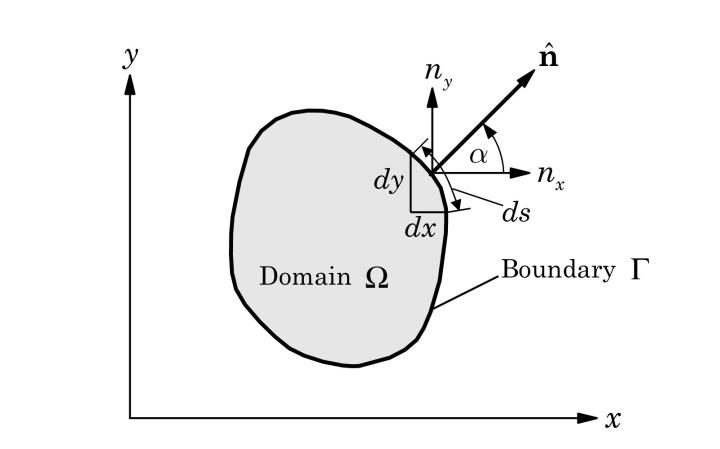
\includegraphics[width=0.5 \linewidth]{Figure/fig25} 		
		\end{figure}
	\begin{itemize}
		\item In the case of heat transfer through an anisotropic medium, aij denotes the conductivity and qn is the normal heat flux
		
	\end{itemize}
	\end{frame}


	\begin{frame}{FEM}
		\begin{itemize}
			\item The weak form states that u should be atleast linear in both x and y
			\item $u_h^e = \sum u_iN_i(x,y)$ with $N_i(x_j,y_j) = \delta_{ij} $ and $\sum_j N_j(x,y)=1$
			\begin{figure}
				\centering
				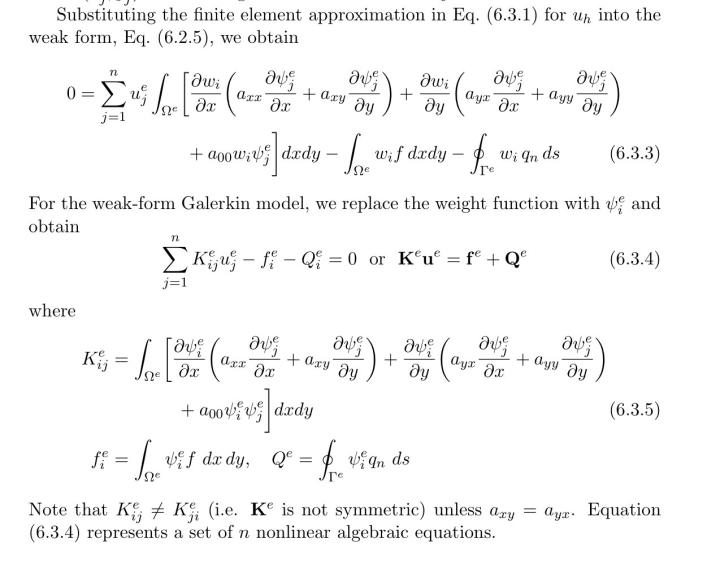
\includegraphics[width=0.8 \linewidth]{Figure/fig26} 		
			\end{figure}	
		\end{itemize}
	\end{frame}


	\begin{frame}
		\begin{itemize}
			\item The equations have to be solved by nonlinear methods
			\item The tangent T is given in page 271
		\end{itemize}
	\end{frame}


	\begin{frame}{Axisymmetric problems}
		\begin{itemize}
			\item The differential equation in cylindrical coordinate system (r,$\theta,z$)
			\begin{equation}
				-\frac{1}{r}\frac{\partial}{\partial r}\left(ra_{rr}\frac{\partial u}{\partial r} \right)
				- \frac{1}{r^2}\frac{\partial}{\partial \theta}\left(a_{\theta\theta}\frac{\partial u}{\partial \theta} \right)
				- \frac{\partial}{\partial z}\left(a_{zz}\frac{\partial u}{\partial z} \right) = f
			\end{equation} 
			\item where u,f and the coefficients are a function of (r,$\theta,z$)
			\item Dependant on the coefficents, boundary conditions and load f the problem can be made to 2D or even 1D
			\item If the cylinder is very long and stuff dont vary and depend on z, then we can assume a disk. No also if there is independance from $\theta$ then we can even just do a radial line \footnote{We just remove the derivatives in the equations where the change will be zero}
			\begin{figure}
				\centering
				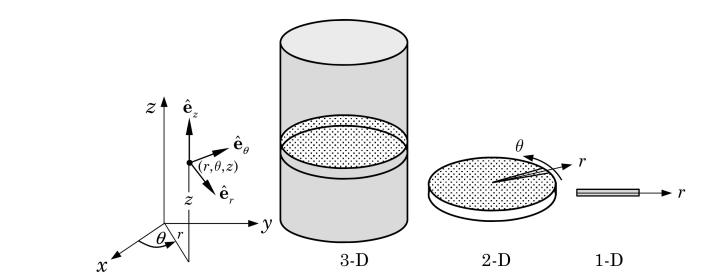
\includegraphics[width=0.8 \linewidth]{Figure/fig27} 		
			\end{figure}
		\end{itemize}
	\end{frame}


	\begin{frame}{FEM}
		\begin{itemize}
			\item Suppose all the variables are not dependant on $\theta$, therefore we would get something like a plane and the Governing differential equation will be
			\begin{equation}
				-\frac{1}{r}\frac{\partial}{\partial r}\left(ra_{rr}\frac{\partial u}{\partial r} \right)
				- \frac{\partial}{\partial z}\left(a_{zz}\frac{\partial u}{\partial z} \right) = f(r,z)
			\end{equation}
			\item The weighted statement and weak form (Using greens theorem) will be given as :
			\begin{equation}
			\begin{aligned}
			 0 = \int_A w_i \left[ 	-\frac{1}{r}\frac{\partial}{\partial r}\left(ra_{rr}\frac{\partial u}{\partial r} \right)
			 - \frac{\partial}{\partial z}\left(a_{zz}\frac{\partial u}{\partial z} \right) - f(r,z)\right] rdrdz \\
			 = \int_A \left[ a_{rr}(r,z,u_h) \frac{\partial w_i}{\partial r}\frac{\partial u_h}{\partial r}
			 + a_{zz}(r,z,u_h) \frac{\partial w_i}{\partial z} \frac{\partial u_h}{\partial z}\right] rdrdz - \int_A w_if(r,z)rdrdz - \int_S w_iq_n ds 
			\end{aligned}
			\end{equation}
			where $q_n = r\left[ a_{rr} \frac{\partial u_h}{\partial r}n_r + a_{zz}\frac{\partial u_h}{\partial z} n_z\right]$
			\item And we get $\ve{Ku = f+Q = F}$
			\item Remember the shape functions are functions of N(r,z)	
	\end{itemize}
	\end{frame}


	\begin{frame}{Numerical integration}
		\begin{itemize}
			\item
			\begin{figure}
				\centering
				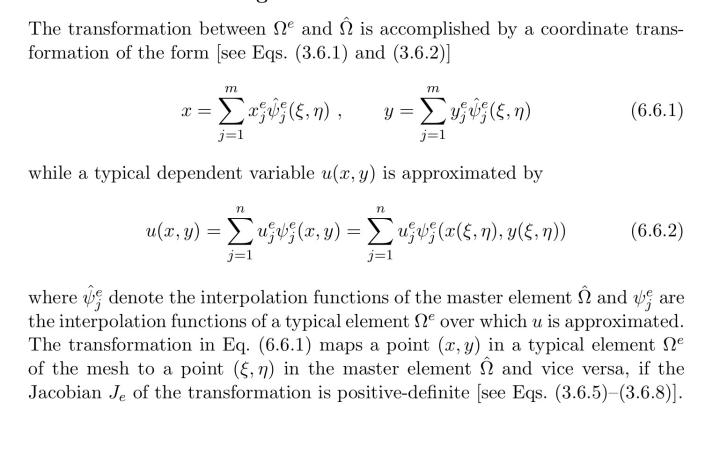
\includegraphics[width=0.9 \linewidth]{Figure/fig28} 		
			\end{figure} 
			
		\end{itemize}
	\end{frame}

	
	\begin{frame}{Gauss quad - coordinate change}
		\begin{itemize}
			\item Remember that we have to we have to transform the integral domain to the master element so that Gauss quadrature can be usd. The derivatives in the original geometry are also expressed with respect to $\xi,\eta$ given by
			\begin{equation}
			\mat{\frac{\partial N_i}{\partial dx}; ;\frac{\partial N_i}{\partial dy} } = \ve{J^{-1}} \mat{\frac{\partial N_i}{\partial d\xi}; ;\frac{\partial N_i}{\partial d\eta} } 
			\end{equation}
			where $\ve{J} = \mat{\frac{\partial x}{\partial \xi}, \frac{\partial y}{\partial \xi}; , ; \frac{\partial x}{\partial \eta}, \frac{\partial y}{\partial \eta}} =
			\mat {\sum x_i \frac{\partial N_i}{\partial \xi}, \sum y_i \frac{\partial N_i}{\partial \xi} ; , ; 
			\sum x_i \frac{\partial N_i}{\partial \eta}, \sum y_i \frac{\partial N_i}{\partial \eta}} = \mat{\frac{\partial N_1}{\partial \xi}, \frac{\partial N_2}{\partial \xi}, .... ,\frac{\partial N_m}{\partial \xi} ; , , ,;
			\frac{\partial N_1}{\partial \eta}, \frac{\partial N_2}{\partial \eta}, ...., \frac{\partial N_m}{\partial \eta} }
	 		\mat{x_1, y_1; , ; x_2, y_2; , ; \vdots, \vdots; x_m,y_m}$ 
	 		\item If the same shape functionsa re used for the geometry and field variable, we say its isoparametric
		\end{itemize}
	\end{frame}


	\begin{frame}
		\begin{figure}
			\centering
			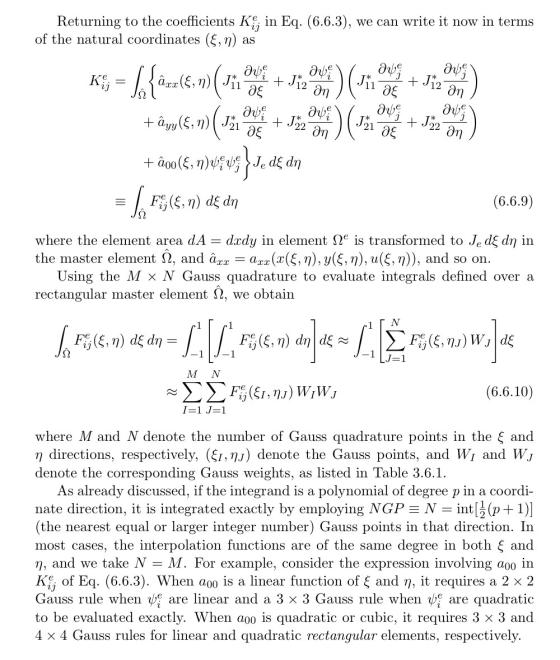
\includegraphics[width=0.6 \linewidth]{Figure/fig29} 		
		\end{figure} 
	where J* are the components of the inverse jacobian
	\end{frame}


	\section{Time dependant problems}
	
	\begin{frame}{Time dependacy}
		Will have to read later!!
	\end{frame}


\end{document}
